\documentclass[9pt]{beamer}
\usepackage[utf8]{inputenc}
\usepackage[T1]{fontenc}
\usepackage{helvet}
\usepackage{fixltx2e}
\usepackage{graphicx}
\usepackage{grffile}
\usepackage{longtable}
\usepackage{wrapfig}
\usepackage{rotating}
\usepackage[normalem]{ulem}
\usepackage{amsmath}
\usepackage{textcomp}
\usepackage{amssymb}
\usepackage{capt-of}
\usepackage{hyperref}
\usepackage{subfig}
\captionsetup[subfloat]{%
font=footnotesize,
indention=10pt}

\usetheme{inria}

\author{Loris Lucido} \date{26 septembre 2016} \title{Ordonnancement
  d'applications de type stencil sur cluster hybrides CPU/GPU}
\subtitle{Université de Bordeaux - LaBRI - INRIA Bordeaux Sud-Ouest - Équipe
  \textsc{Storm}}

% \AtBeginSection[]{
%   \begin{frame}[plain]
%     \partpage
%   \end{frame}
% }

\begin{document}

\begin{frame}[plain]
  \titlepage
\end{frame}

% \begin{frame}{\textcolor{inriaGrey}{Sommaire}}
%   \tableofcontents
% \end{frame}

\section{Introduction au sujet}

\begin{frame}{Domaine du Calcul Haute Performance}
  \vfill
  \begin{itemize}
  \item Résoudre un problème
    \vfill
    \begin{itemize}
    \item de plus en plus rapidement
      \vfill
    \item de taille de plus en plus grande
    \end{itemize}
    \vfill
  \item Application de simulation en :
    \vfill
    \begin{itemize}
    \item climatologie
      \vfill
    \item aérospatiale
      \vfill
    \item dynamique moléculaire
    \end{itemize}
  \end{itemize}
\end{frame}

\begin{frame}{Présentation de l'équipe \textsc{STORM}}
  \vfill
  \textit{STatic Optimizations Runtime Methods}, trois axes de recherche :
  \vfill
  \begin{itemize}
  \item Langage de haut niveau spécifique à un domaine (\textit{e.g. QIRAL})
  \vfill
  \item Outils d'analyse de performance et d'aide à l'optimisation (\textit{e.g. MAQAO})
  \vfill
  \item Support d'exécution pour des calculateurs hétérogènes (\textit{StarPU})
  \end{itemize}
  \vfill
\end{frame}

\begin{frame}{Architecture hétérogène}
  \vfill
  \begin{minipage}{0.45\textwidth}
    \begin{itemize}
    \item<1-> Des dizaines de cœurs par processeurs
      \vfill
    \item<2-> Plusieurs processeurs par machine
      \vfill
    \item<3-> Plusieurs cartes graphiques dédiées au calcul :
      \begin{itemize}
      \item parallélisme massif
      \end{itemize}
    \end{itemize}
    \vfill
  \end{minipage} \hfill
  \begin{minipage}{0.50\textwidth}
    \centering
    \includegraphics[width=0.7\linewidth]{img/arch-1.pdf}<1>
    \includegraphics[width=1\linewidth]{img/arch-2.pdf}<2>
    \includegraphics[width=1\linewidth]{img/arch-3.pdf}<3>
  \end{minipage} \hfill
\end{frame}

\begin{frame}{Architecture hétérogène}
  \begin{figure}
    \centering
    \includegraphics[width=0.5\linewidth]{img/arch-4.pdf}
    \caption{Topologie mémoire d'une machine avec deux cartes graphiques.}
  \end{figure}
  \vfill
  Carte graphique dédiée au calcul :
  \vfill
  \begin{itemize}
  \item<2-> Mémoire dédiée en quantité limitée
    \vfill
  \item<3-> Pas d'accès direct à la mémoire principale
  \end{itemize}
\end{frame}

\begin{frame}{Le support d'exécution (ou \textit{Runtime}) StarPU}
  \vfill
  \begin{itemize}
  \item Entre le système d'exploitation et l'application
    \vfill
  \item Exploite une architecture :
    \vfill
    \begin{itemize}
    \item portable et générique
      \vfill
    \item paradigme de programmation parallèle en tâches
    \end{itemize}
    \vfill
  \item Stratégies d'ordonnancement (ordonnanceur)
  \end{itemize}
  \vfill
\end{frame}

\section{Contexte}

\begin{frame}{\textcolor{inriaGrey}{Programmation parallèle en tâches}}
  \vfill
  \begin{itemize}
    \vfill
  \item Découpage du problème en sous-ensembles : tâches \vfill
  \item Exécution parallèle des tâches sur différentes unités de calcul \vfill
  \item Dépendances de données entre les tâches \vfill
    \begin{figure}
      \centering
      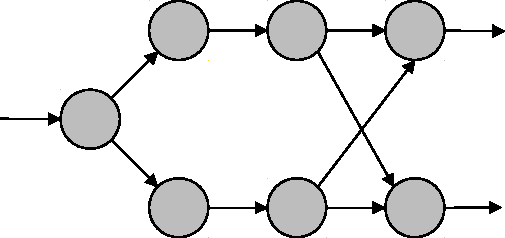
\includegraphics[width=0.5\linewidth]{img/task-deps.pdf}
      \caption{Graphe de dépendances de tâches.}
    \end{figure}
    \vfill
  \end{itemize}
\end{frame}

\begin{frame}{\textcolor{inriaGrey}{Ordonnancement des tâches par le support d'exécution}}
  \begin{itemize}
  \item Ordonnancement du graphe de tâches sur les différents unités de calcul
    ou ouvriers : \vfill
    \begin{itemize}
    \item cœurs CPU (processeur) \vfill
    \item GPU (carte graphique)
    \end{itemize}
      \vfill
    \item Choisir le «meilleur ouvrier» pour une tâche donnée \vfill
  \item Transférer les résultats des calculs \vfill
  \end{itemize}
\end{frame}

\begin{frame}{\textcolor{inriaGrey}{Applications stencils}}
  \vfill
  Qu'est-ce qu'une application stencil ?
  \vfill
  \begin{itemize}
    \item Stencil : motif ou pochoir que l'on applique par répétition sur
      l'ensemble du domaine étudié
  \end{itemize}
  \vfill
  \begin{figure}
    \centering
    \includegraphics[width=0.6\linewidth]{img/5-points-stencil.pdf}
    \caption{Exemples de stencil 5-points en 2D et 1D.}
  \end{figure}
  \vfill
  \begin{itemize}
  \item<2-> Mise à jour d'une cellule en fonction du voisinage, schéma appliqué
    «simultanément» sur un ensemble de cellules \vfill
\end{itemize}
\end{frame}

\begin{frame}{\textcolor{inriaGrey}{Applications stencils}}
  \begin{figure}
    \centering
    \includegraphics[width=0.5\linewidth]{img/grid-0.pdf}<1>
    \includegraphics[width=0.5\linewidth]{img/grid-1.pdf}<2>
    \includegraphics[width=0.4\linewidth]{img/grid-2.pdf}<3>
    \includegraphics[width=0.4\linewidth]{img/grid-3.pdf}<4>
    \includegraphics[width=0.4\linewidth]{img/grid-4.pdf}<5>
    \includegraphics[width=0.5\linewidth]{img/grid-5.pdf}<6>
    \includegraphics[width=0.5\linewidth]{img/grid-6.pdf}<7>
    \includegraphics[width=0.5\linewidth]{img/grid-7.pdf}<8>
    \caption{Exemple d'application de stencil.}
  \end{figure}
  \vfill
  \begin{itemize}
  \item<2-> Ratio nombre d'accès mémoires par mise à jour très élevé \vfill
  \item<8-> Dimension temporelle construite avec des \textit{itérations}
  \end{itemize}
  \vfill
\end{frame}

\begin{frame}{\textcolor{inriaGrey}{Objectifs généraux du stage}}
  \vfill
  \begin{itemize}
  \item<1-> Travail sur le recouvrement des transferts mémoires par du calcul
    \vfill
  \item<2-> Travail sur la localité (spatiale et temporelle) des données \vfill
  \item<3-> Problématique du stage : \newline Est-ce que les stratégies
    d'ordonnancement génériques du support d'exécution \textit{StarPU} sont
    adaptées à des applications stencil, où la localité des données est
    cruciale ?
  \end{itemize}
  \vfill
\end{frame}

\begin{frame}{\textcolor{inriaGrey}{Environnement de test : exécution simulée}}
    \begin{itemize}
    \item reproductible \vfill
    \item total contrôle sur les paramètres : \vfill
      \begin{itemize}
      \item durée d'une tâche \vfill
      \item temps de transfert \vfill
      \item architecture de la machine
      \end{itemize}
    \end{itemize}
\end{frame}

\begin{frame}{\textcolor{inriaGrey}{Résumé de la contribution}}
  \vfill
  \begin{itemize}
  \item<1-> Outil de visualisation pour observer la localité des données
    \vfill
  \item<2-> Méthode de référence : construction d'un ordre de soumission de
    tâches optimisé pour stencil \vfill
  \item<3-> Évaluation des ordonnanceurs de \textit{StarPU} pour des
    applications stencils : \vfill
    \begin{itemize}
    \item<4-> temps de calcul d'une tâche = 2 x temps de transfert \vfill
    \item<5-> taille de problème > mémoire des cartes graphiques \vfill
    \item<6-> problème de déséquilibre de charge
    \end{itemize}
    \vfill
  \item<7-> Assemblage d'un ordonnanceur qui exploite l'information de localité
    des données
  \end{itemize}
  \vfill
\end{frame}

\section{Méthode de référence pour l'évaluation}

\begin{frame}{\textcolor{inriaGrey}{Le cas à éviter : aucune localité des données}}
  \begin{figure}
    \centering
    \hspace*{\fill}
    \includegraphics[width=0.45\linewidth]{img/worst-nolimit.png}
    \hspace*{\fill}
    \includegraphics[width=0.55\linewidth]{img/xpm-legend-gpu1.pdf}
    \hspace*{\fill}
    \newline \vfill
    \includegraphics[width=1\linewidth]{img/worst-limit.png}<2->
    \vfill
    \caption{Diagramme en temps d'une exécution avec soumission de tâches naïve
      sur un GPU.}
  \end{figure}
\end{frame}

\begin{frame}{\textcolor{inriaGrey}{Algorithme cache oublieux (\textit{oblivious})}}
  \vfill
  \begin{itemize}
  \item Matteo \textsc{Frigo} et Volker \textsc{Strumpen} : « Cache Oblivious
    Stencil Computations » \vfill
  \item<2-> Limite les chargements mémoires hors cache (\textit{cache misses})
    \vfill
  \item<3-> Favorise la réutilisation des données \vfill
  \item<4-> Découple l'optimisation du paramètre «taille du cache»
  \end{itemize}
  \vfill
\end{frame}

\begin{frame}{\textcolor{inriaGrey}{Soumission de tâches cache oublieux}}
  \vfill
  Une soumission cache oublieuse de tâches au support d'exécution permet de :
  \vfill
  \begin{itemize}
  \item<2-> Favoriser la localité des données \vfill
  \item<3-> Limiter les transferts mémoires entre cartes graphiques et mémoire
    principale
  \end{itemize}
  \vfill
  \begin{figure}
    \centering
    \includegraphics[width=1\linewidth]{img/co-gpu1.png}
    \caption{Diagramme en temps d'une exécution avec soumission de tâches cache
      oublieux sur un GPU.}
  \end{figure}
  \begin{figure}
    \centering
    \includegraphics[width=0.5\linewidth]{img/xpm-legend-gpu1-nt.pdf}
  \end{figure}
\end{frame}

\begin{frame}{\textcolor{inriaGrey}{Version parallèle - respect des dépendances}}
  \vfill
  \begin{figure}
    \centering
    \includegraphics<1->[width=1\linewidth]{img/co-gpu2-nomirror.pdf}
  \end{figure}
  \begin{figure}
    \centering
    \includegraphics<2->[width=0.8\linewidth]{img/co-gpu2-mirror.png}
    \caption{Diagramme en temps d'une exécution avec soumission parallèle de
      tâches cache oublieux sur deux GPU.}
  \end{figure}
  \begin{figure}
    \centering
    \includegraphics[width=0.6\linewidth]{img/xpm-legend-gpu2.pdf}
  \end{figure}
  \vfill
\end{frame}

\section{Ordonnanceur \texttt{dmdar} - localité des données}

\begin{frame}{\textcolor{inriaGrey}{Ordonnancement d'une tâche pour l'ordonnanceur \texttt{dmdar}}}
  \begin{minipage}{0.65\textwidth}
    \begin{figure}
      \centering
      \includegraphics[width=1\linewidth]{img/sched_dmdar.pdf}
    \end{figure}
  \end{minipage} \hfill
  \begin{minipage}{0.3\textwidth}
    \begin{itemize}
    \item Modèle de performance (temps de calcul des tâches)
    \item Temps de transfert
    \item Tri des tâches par données prêtes
    \end{itemize}
  \end{minipage}
\end{frame}

\begin{frame}{\textcolor{inriaGrey}{Ordonnancement d'une tâche pour l'ordonnanceur \texttt{dmda}}}
  \begin{minipage}{0.65\textwidth}
    \begin{figure}
      \centering
      \includegraphics[width=1\linewidth]{img/sched_dmda.pdf}
    \end{figure}
  \end{minipage} \hfill
  \begin{minipage}{0.3\textwidth}
    \begin{itemize}
    \item Modèle de performance (temps de calcul des tâches)
    \item Temps de transfert
    \end{itemize}
  \end{minipage}
\end{frame}

\begin{frame}{\textcolor{inriaGrey}{Choix du meilleur ouvrier pour une tâche}}
  \begin{figure}
\hspace*{\fill}
\subfloat[État initial des files de tâches.]
  {\includegraphics[width=0.3\linewidth]{img/sched_dmda_1.pdf}}
\hspace*{\fill}
\subfloat[Temps de calcul.]
  {\includegraphics[width=0.3\linewidth]{img/sched_dmda_2.pdf}}
\hspace*{\fill}
\newline
\hspace*{\fill}
\subfloat[Temps de transfert.]
  {\includegraphics[width=0.3\linewidth]{img/sched_dmda_5.pdf}}
\hspace*{\fill}
\subfloat[Choix de l'ouvrier idéal.]
  {\includegraphics[width=0.3\linewidth]{img/sched_dmda_6.pdf}}
\hspace*{\fill}
\caption{Recherche d'une date de terminaison minimale.}
\end{figure}
\end{frame}

\begin{frame}{\textcolor{inriaGrey}{Comparaison avec la méthode de référence}}
  \begin{figure}
    \centering
    \includegraphics[width=0.7\linewidth]{exp/perf_gpu2_limit200.pdf}
    \caption{Évolution du temps d'exécution en fonction de la taille du problème
      - 2 GPU, limite mémoire fixée à 200MB par GPU.}
  \end{figure}
  \vfill
  \begin{itemize}
  \item<2-> Souligne l'importance du recouvrement des transferts mémoires
  \vfill
  \item<3-> \texttt{dmdar} ne casse pas les situations favorables
  \vfill
  \item<4-> Performances encore trop éloigné de l'idéal (1.5x plus lent)
  \end{itemize}
  \vfill
\end{frame}

\begin{frame}
  \begin{figure}
    \begin{minipage}{0.3\textwidth}
      \centering
      \includegraphics[width=0.75\linewidth]{img/dmdar-iter-gpu2.png}
    \end{minipage} \hfill
    \begin{minipage}{0.65\textwidth}
      Objectif : limiter la quantité de frontières \vfill
      \includegraphics[width=0.55\linewidth]{img/xpm-legend-iter-gpu2.pdf}
    \end{minipage} \hfill
    \caption{%
      \label{fig:dmdar-iter-gpu2}%
      Diagramme en itérations d'une exécution de \texttt{dmdar}. 2 GPU, taille
      du problème 1800MB, limite mémoire fixée à 200MB par GPU.}
  \end{figure}
\end{frame}

\begin{frame}
  \begin{figure}
    \centering
    \vfill
    \includegraphics[width=1\linewidth]{img/dmdar-gpu2.pdf}
    \newline
    \vfill
    \includegraphics[width=0.6\linewidth]{img/xpm-legend-gpu2.pdf}
    \vfill
    \caption{%
      \label{fig:dmdar-gpu2}%
      Diagramme en temps - Échantillon d'exécution de \texttt{dmdar}. 2 GPU,
      taille du problème 1800MB, limite mémoire fixée à 200MB par GPU.}
  \end{figure}
  \vfill
\end{frame}

\section{Conclusion}

\begin{frame}{\textcolor{inriaGrey}{Résumé des points importants}}
  \begin{itemize}
  \item Stencil :
    \vfill
    \begin{itemize}
    \item Ratio accès mémoire par mises à jour élevé \vfill
    \item Observer la localité des données : outil adapté \vfill
    \end{itemize}
  \item Évaluer les ordonnanceurs :
   \vfill
    \begin{itemize}
    \item Méthode de référence : algorithme cache oublieux pour stencil \vfill
    \item Est-ce que les ordonnanceurs (génériques) de \textit{StarPU} sont
      adaptés à des stencils ?
    \end{itemize}
  \end{itemize}
\end{frame}

\begin{frame}{\textcolor{inriaGrey}{Conclusion}}
  \vfill
  Bilan :
  \vfill
  \begin{itemize}
  \item Le support d'exécution \textit{StarPU}, performances satisfaisantes :
  \vfill
    \begin{itemize}
    \item encore trop éloignées de l'idéal
    \item générique et portable
    \end{itemize}
  \end{itemize}
  \vfill
  Améliorations :
  \vfill
  \begin{itemize}
  \item Ordonnanceur : améliorer l'amorce \vfill
  \item Visualisation pour stencils à dimension arbitraire (2D, 3D, etc.) \vfill
  \item Test d'un vrai stencil (e.g. application de simulation nucléaire)
  \end{itemize}
  \vfill
\end{frame}

\begin{frame}{\textcolor{inriaGrey}{Perspectives}}
  \vfill
  \begin{itemize}
  \item \textit{Out of core} : plus de place en mémoire principale
    \begin{itemize}
    \item Rapatriement en mémoire du disque dur
    \end{itemize}
    \vfill
  \item Programmation distribuée en réseau (\textit{Message Passing Interface})
  \end{itemize}
  \vfill
\end{frame}

\end{document}

% programme de test : env 600l de code
% outils de visualisation : env 600l de code
